\begin{savequote}[45mm]
\ascii{Any fool can write code that a computer can understand. Good programmers write code that humans can understand.}
\qauthor{\ascii{- Martin Flower}}
\end{savequote}

\chapter{聚集参数} 
\label{ch:param-collector}

\begin{content}

本章重点讨论收集测试结果的实现机制,重构趋向\emph{聚集参数}模式。聚集参数由\ascii{Kent Beck}在其经典著作《实现模式》中引入的,他将\emph{聚集参数}抽象为一个对象,并传递给不同的函数,以便在函数调用链中聚集结果。

\end{content}

\section{收集器}

\begin{content}

在之前的测试用例中,为了统计测试用例的运行数目,在匿名命名空间内引入计数器\ascii{num}。当某个用例被执行时,执行计数器的累加操作。显而易见,计数器游离在对象之外是极为危险的,即使该计数器已经被限制在匿名命名空间内。因为,在其可见的作用域内都有可能被他人修改。

这是一种脆弱的设计,用户需要小心地维护计数器的初始化,及其精细控制计数器累加的时机。一则容易引入不经意的错误,二则使得操作计数器的代码散乱到各个子类覆写的\ascii{runTest}之中。

\begin{nodiff}{test/mars/core/TestSuiteSpec.cc}
 \begin{c++}
#include <mars/core/TestCase.h>
#include <gtest/gtest.h>

namespace {
  int num = 0;

  struct FooTest : TestCase {
  private:
    void runTest() override {
      num++;
    }
  };

  struct TestCaseSpec : testing::Test {
  private:
    void SetUp() override {
      num = 0;  // IMPORTANT: reset counter.
    }

  protected:
    void run(::Test& test) {
      test.run();
    }
  };
}

TEST_F(TestCaseSpec, run_one_simple_test) {
  FooTest test("simple test");
  run(test);
  ASSERT_EQ(1, num);
}
 \end{c++}
\end{nodiff}

\subsection{提取对象}

为了消除这个不稳定的设计,将计数器移入到对象。一则方便计数器的初始化,二则限制计数器的作用域。因此,此处引入\ascii{TestResult}对象,它负责管理计数器的生命周期,及其收集测试结果,并对外暴露查询接口\ascii{runCount}。

另外,并没有直接在既有的\ascii{TestCase::run}增加聚集参数\ascii{TestResult};而是新增加成员函数\ascii{TestCase::runWith},其携带聚集参数\ascii{TestResult}。否则,将导致大量用例编译失败,因为修改\ascii{TestCase::run}声明,将导致\ascii{Test::run, TestSuite::run},及其所有引用点的联动修改。想要通过测试,需要付出很大的努力。因此,此处保守地新建成员函数\ascii{runWith},将所有修改局部于\ascii{TestCase}内部,有效控制变更波及的影响。

\begin{nodiff}{test/mars/core/TestSuiteSpec.cc}
 \begin{c++}
#include <mars/core/TestCase.h>
#include <mars/core/TestResult.h>
#include <gtest/gtest.h>

TEST(TestCaseSpec, run_one_simple_test) {
  TestResult result;
  TestCase test;
  
  test.runWith(result);
  ASSERT_EQ(1, result.runCount());
}
 \end{c++}
\end{nodiff}

\subsubsection{通过编译}

为了快速通过测试,新建头文件\ascii{TestResult.h},并对外提供查询接口\ascii{runCount}。

\begin{nodiff}{include/mars/core/TestResult.h}
 \begin{c++}
struct TestResult {
  int runCount() const;
};
 \end{c++}
\end{nodiff}

新增\ascii{TestCase::runWith}的接口声明,其持有聚集参数\ascii{TestResult}。

\begin{nodiff}{include/mars/core/TestCase.h}
 \begin{c++}
#include <mars/core/Test.h>
#include <mars/core/TestFixture.h>

struct TestResult;

struct TestCase : Test, private TestFixture {
  using Test::Test;

  void runWith(TestResult&);

private:
  void run() override;

private:
  virtual void runTest() {}
};
 \end{c++}
\end{nodiff}

至此,编译通过。

\subsubsection{通过测试}

为了尽快通过测试,伪实现\ascii{TestResult::runCount},直接返回\ascii{1}。

\begin{nodiff}{src/mars/core/TestResult.cc}
 \begin{c++}
#include <mars/core/TestResult.h>

int TestResult::runCount() const {
  return 1;
}
 \end{c++}
\end{nodiff}

暂且将\ascii{TestCase::runWith}的实现委托给\ascii{TestCase::run}。

\begin{nodiff}{src/mars/core/TestCase.cc}
 \begin{c++}
#include <mars/core/TestCase.h>

void TestCase::run() {
  setUp();
  runTest();
  tearDown();
}

void TestCase::runWith(TestResult&) {
  run();
}
 \end{c++}
\end{nodiff}

通过测试。

\begin{figure}[H]
\centering
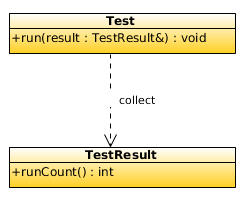
\includegraphics[width=0.4\textwidth]{figures/xunit/test-result.png}
\caption{聚集参数:收集测试结果}
 \label{fig:test-tree}
\end{figure}

\subsection{提取对象}

\end{content}

\section{统计器}

\begin{content}

% \ascii{TestResult::runCount}在运行时,通过监听接口统计测试用例的数目。事实上,也可以遍历用例树,直接统计测试用例的数目。构造一个失败的用例,观察如何统计测试用例数目。

% \subsection{测试用例}

% \begin{leftbar}
%  \begin{c++}[caption={\ttfamily{test/mars/core/TestSuiteSpec.cc}}]
% #include <gtest/gtest.h>
% #include "mars/core/TestCase.h"
% #include "mars/core/TestSuite.h"
% #include "mars/core/TestResult.h"

% namespace {
%   struct TestSuiteSpec : testing::Test {
%     void run(::Test& test) {
%       test.run(result);
%     }

%     int countTestCases(::Test& test) {
%       return test.countTestCases();
%     }

%   protected:
%     TestResult result;
%   };
% }

% TEST_F(TestSuiteSpec, run_multi_test_cases_using_test_suite) {
%   TestSuite suite;
%   suite.add(new TestCase);
%   suite.add(new TestCase);

%   run(suite);

%   ASSERT_EQ(2, countTestCases(suite));
% }
%  \end{c++}
% \end{leftbar}

% \subsection{定义虚接口}

% 增加\ascii{Test::countTestCases}纯虚接口。

% \begin{leftbar}
%  \begin{c++}[caption={\ttfamily{include/mars/core/Test.h}}]
% #include <string>

% struct TestResult;

% struct Test {
%   explicit Test(const std::string& name = "");
%   const std::string& getName() const;

%   virtual ~Test() {}
%   virtual int countTestCases() const = 0;
%   virtual void run(TestResult&) = 0;

% private:
%   std::string name;
% };
%  \end{c++}
% \end{leftbar}

% \subsection{实现虚接口}

% \ascii{TestCase::countTestCases}覆写行为直接返回\ascii{1}。

% \begin{leftbar}
%  \begin{c++}[caption={\ttfamily{src/mars/core/TestCase.cc}}]
% int TestCase::countTestCases() const {
%   return 1;
% }
%  \end{c++}
% \end{leftbar}

% \ascii{TestSuite::countTestCases}覆写行为完成\ascii{reduce}操作。

% \begin{leftbar}
%  \begin{c++}[caption={\ttfamily{src/mars/core/TestSuite.cc}}]
% int TestSuite::countTestCases() const {
%   auto num = 0;
%   foreach([&num](auto test) {
%     num += test->countTestCases();
%   });
%   return num;
% }
%  \end{c++}
% \end{leftbar}

% 至此,测试通过。相对于\ascii{TestResult::runCount}通过聚集参数实现用例数目的统计,\ascii{TestResult::countTestCases}更加具有可扩展性;并且,\ascii{TestResult}与\ascii{TestCase}的耦合程度更小。

\end{content}

